\section{位置不确定性：从 100 m 圆柱到数百平方公里}

\subsection{30\,000 条轨迹的分支构成}

30\,000 个粒子中，水面/水柱/海底三类目标的占比随时间变化很小
（\figref{fig:unc}b）：约 22\% 最终在水面（S0、S2s 与部分上浮情形），
约 62\% 悬停在水柱（S1、S2b），约 16\% 沉底（S3、S4）。
分支比例稳定意味着搜索的资源分配不应随 $t$ 大幅调整，但\emph{各分支的空间散布}随时间
迅速扩大（\figref{fig:posterior}），这才是搜索难度的来源。

\begin{figure}[H]
\centering
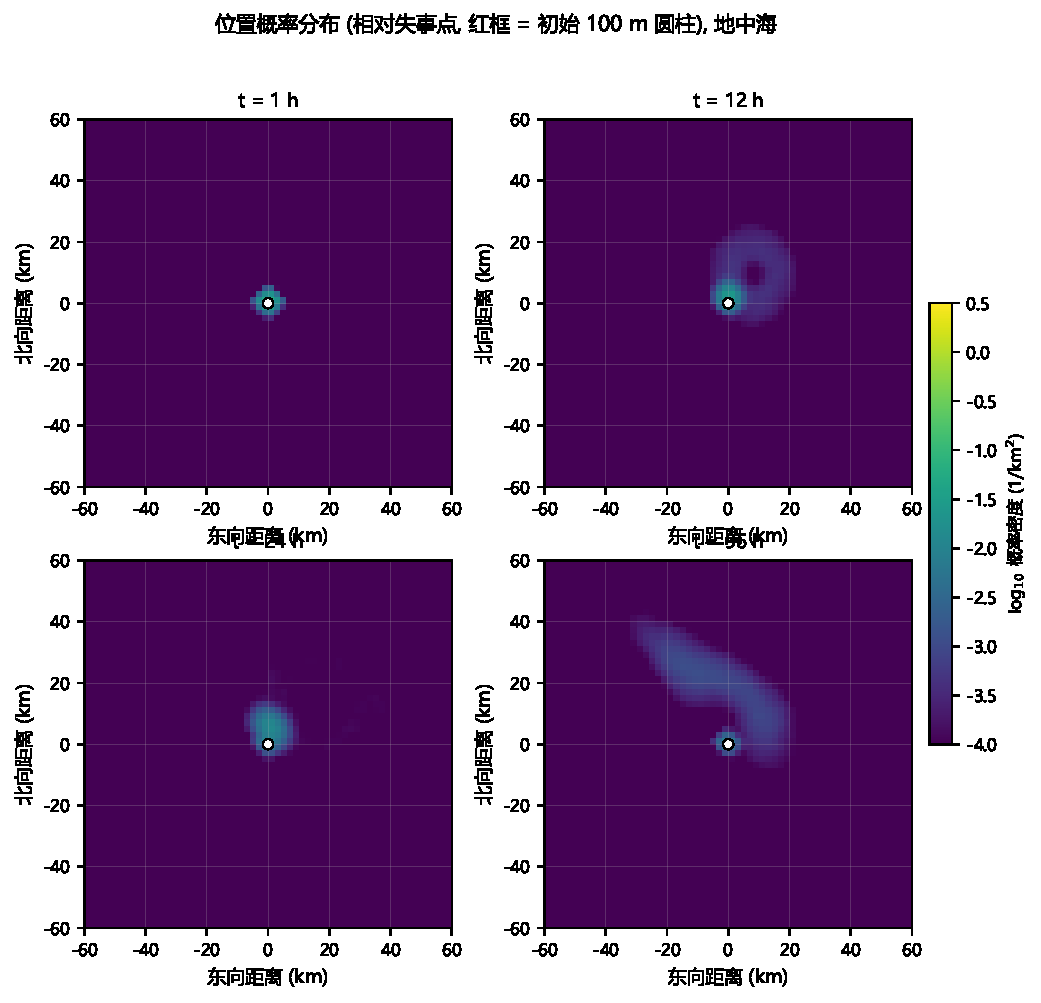
\includegraphics[width=0.60\textwidth]{fig_L1_posterior}
\caption{位置概率分布（相对失事点）。$t=1$ h 时几乎全部集中在初始 100 m 圆柱附近；
12 h 后沿流场形成“水柱分支 + 表面分支”的双峰结构；96 h 时水柱分支向东北方向扩展
约 30--40 km，表面分支则散布到整个区域（图中截断于 $\pm60$ km）。}
\label{fig:posterior}
\end{figure}

\subsection{包含域面积}

把相对失事点的位置概率从高到低累加，得到 50\%/95\% 包含域面积
$A_{50}$、$A_{95}$（\tabref{tab:area}、\figref{fig:unc}a）。这是“搜救方需要搜索多大
范围”的直接度量。

\begin{table}[H]
\centering\small
\caption{包含域面积与漂移距离（主算例，30\,000 粒子）}
\label{tab:area}
\begin{tabular}{@{}rrrrrrr@{}}
\toprule
$t$ (h) & $A_{50}\kmsq$ & $A_{95}\kmsq$ & 水柱 $A_{95}\kmsq$ & 沉底 $A_{95}\kmsq$
& $r_{50}$ (km) & $r_{95}$ (km)\\
\midrule
1  & 16  & 56    & 52   & 56  & 0.3 & 2.0\\
4  & 20  & 112   & 52   & 56  & 1.1 & 7.5\\
12 & 32  & 560   & 76   & 60  & 3.0 & 20.8\\
24 & 60  & 2\,104 & 144  & 60  & 6.3 & 39.6\\
48 & 160 & 8\,328 & 396  & 64  & 13.4 & 62.9\\
72 & 308 & 17\,556 & 804 & 92  & 19.0 & 87.8\\
96 & 488 & 27\,652 & 1\,360 & 120 & 23.7 & 115.4\\
\bottomrule
\end{tabular}
\end{table}

\begin{figure}[H]
\centering
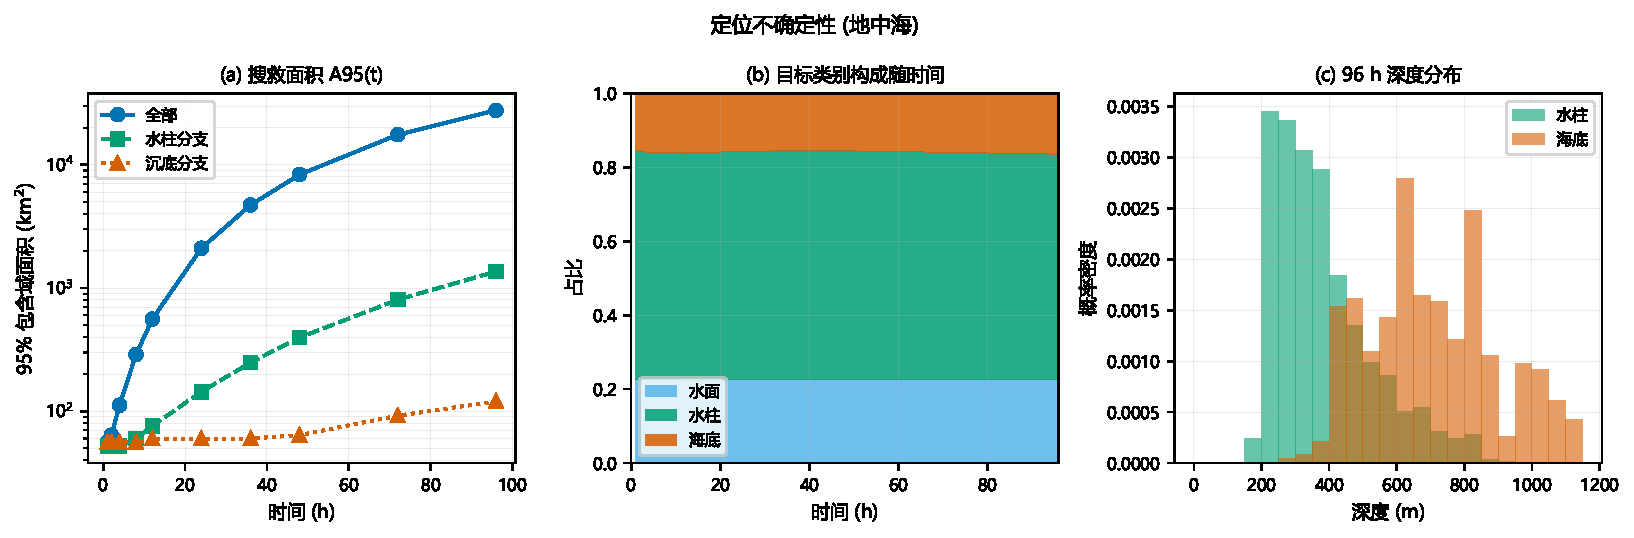
\includegraphics[width=0.80\textwidth]{fig_L2_uncertainty}
\caption{定位不确定性。(a) 包含域面积 $A_{95}$ 随时间：全部/水柱/沉底三个口径；
(b) 目标类别占比随时间；(c) 96 h 深度分布（水柱与沉底分支）。}
\label{fig:unc}
\end{figure}

\subsection{三个直接结论}

\begin{enumerate}[leftmargin=1.8em,itemsep=0pt]
\item \textbf{响应时间是最重要的变量.} $A_{95}$ 在 24 h 内已从 $10^2\km^2$ 量级增至
      $2\,104\km^2$，96 h 达 $27\,652\km^2$（约相当于 $166\times166$ km 的方框）。
      任何搜索装备的单位时间覆盖能力都远小于这个增长速度，因此“多快开始搜”比
      “装备多好”更决定成败；
\item \textbf{水柱分支是搜索主体.} 96 h 时水柱分支 $A_{95}=1\,360\km^2$，占全部面积的
      主导；水面分支由雷达处理、沉底分支面积仅 $120\km^2$，两者的搜索问题相对容易；
\item \textbf{沉底分支面积几乎不增长.} 沉底目标静止，$A_{95}\approx60$--$120\km^2$
      基本由海底地形与滑移决定，是“最难找但范围最小”的一类。
\end{enumerate}

因此定位模型为搜索模型提供的不只是“一条轨迹”，而是\emph{一个逐小时更新的概率地图}：
这正是第 6 节贝叶斯搜索的输入。
